\thispagestyle{hoccungpinone}
\pagestyle{hoccungpi}
\everymath{\color{hoccungpi}}
\graphicspath{{../hoccungpi/pic/}}
\blfootnote{$^1${\color{hoccungpi}Đại học Bách Khoa Hà Nội.}}
\begingroup
\AddToShipoutPicture*{\put(0,616){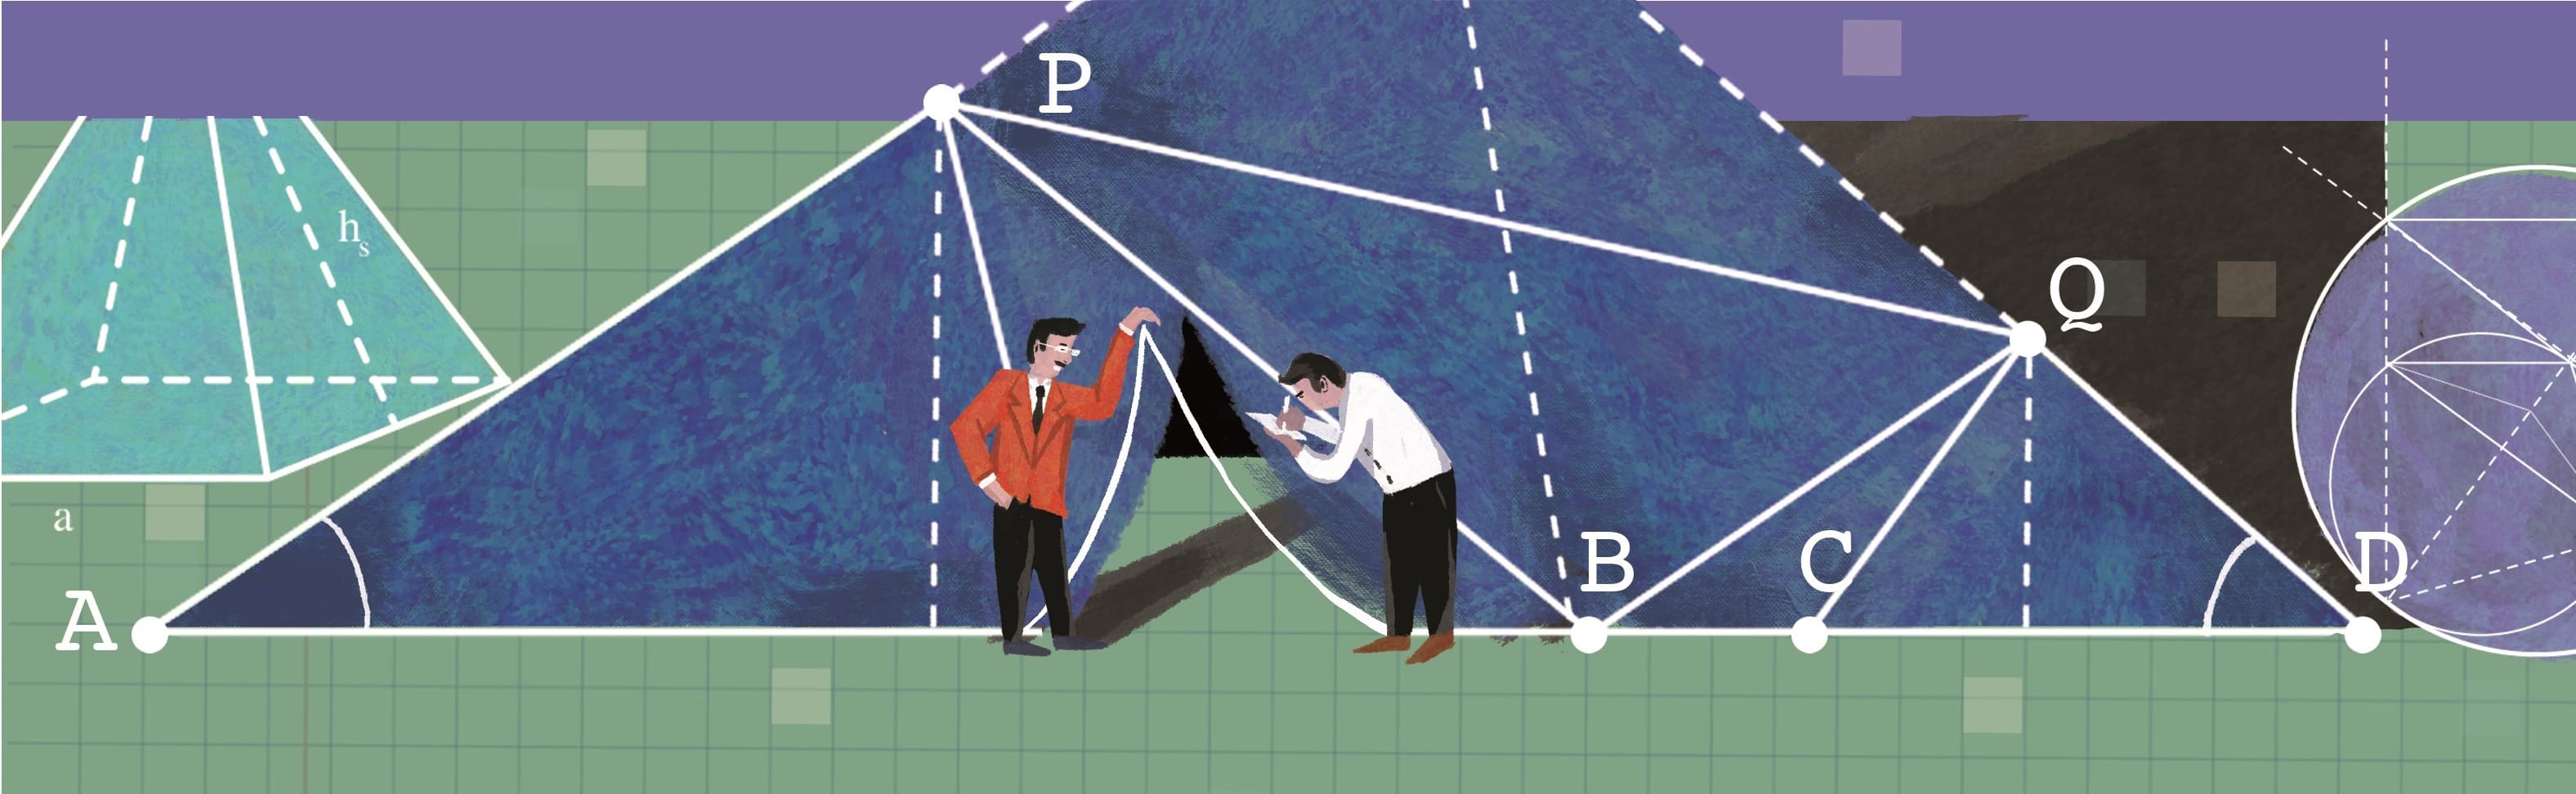
\includegraphics[width=19.3cm]{../bannerhoccungpi}}} 
\AddToShipoutPicture*{\put(60,520){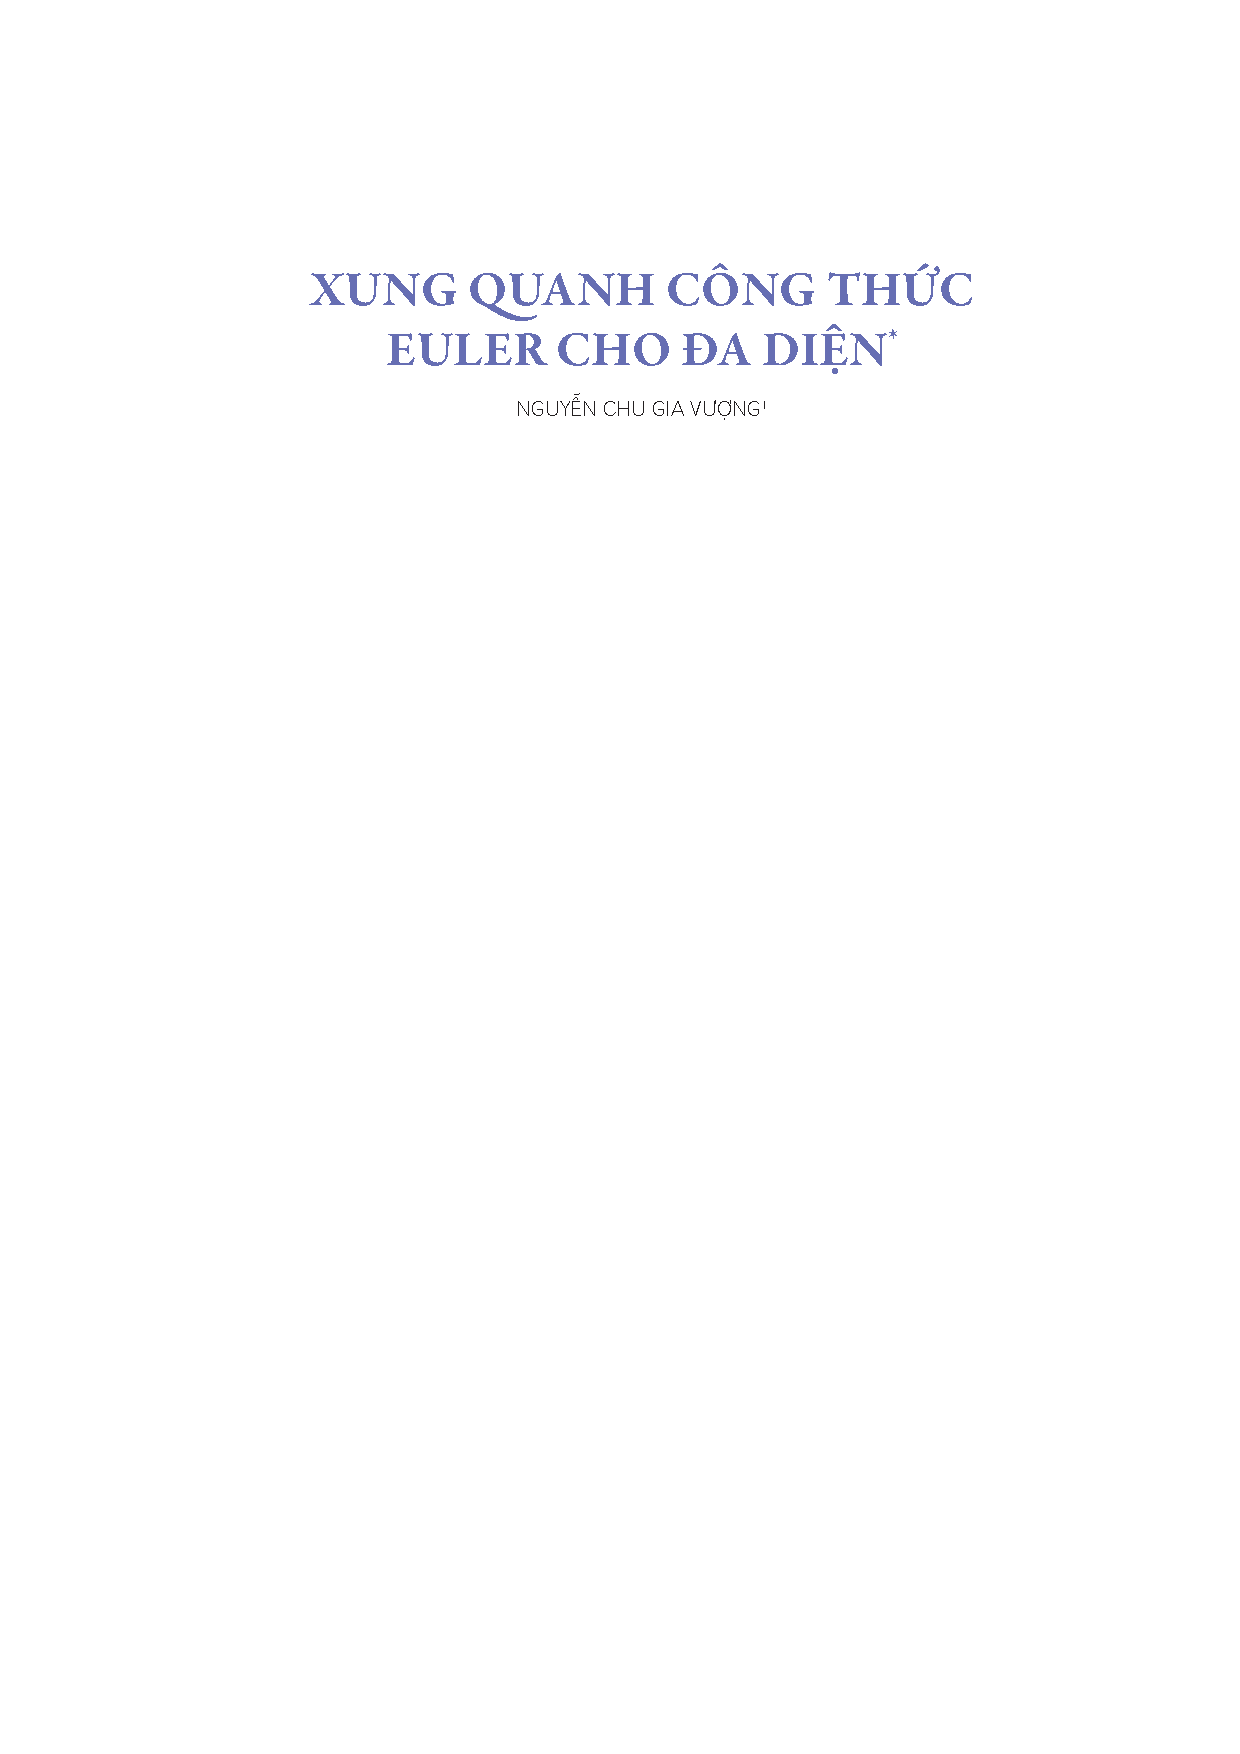
\includegraphics[scale=1]{../tieude.pdf}}} 
\centering
\endgroup
%\def\PIbox#1{\tikz\node[draw,fill=yellow!20,rounded corners,align=justify,text width=.95\linewidth,inner sep=2mm]{#1};}%
%\renewcommand{\qedsymbol}{}
\vspace*{185pt}

\begin{multicols}{2}
	\setlength{\abovedisplayskip}{4pt}
	\setlength{\belowdisplayskip}{4pt}
	Trong bài báo gần đây [$1$], Lukarevski chứng minh bất đẳng thức sau cho mọi tam giác $ABC$:
	\begin{align*}
		\label{BDT1}4R+10r\le AI_A+BI_B+CI_C\le 8R+2r,
	\end{align*}
	trong đó $R$ và $r$ lần lượt là bán kính đường tròn ngoại tiếp và nội tiếp, $I_A,I_B,I_C$ lần lượt là tâm các đường tròn bàng tiếp góc $A,B,C$.  
	\vskip 0.05cm
	Lukarevski đưa ra một chứng minh hình học cho 
	\begin{align*}
		AI_A+BI_B+CI_C\le 8R+2r
	\end{align*}
	và hỏi một chứng minh hình học cho bất đẳng thức 
	\begin{align*}
		4R+10r\le AI_A+BI_B+CI_C. \tag{$1$}
	\end{align*}
	Lukarevski cũng đưa ra phỏng đoán rằng đại lượng $4R+10r$ không thể được thay bởi $5R+8r$. Trong bài báo này, phần $1$ đưa ra một số kết quả quen thuộc trong hình học phẳng, phần $2$ đưa ra một chứng minh hình\linebreak học cho ($1$), và cuối cùng,  phần $3$ đưa ra chứng minh $4$ là hằng số tốt nhất trong ($1$).
	\vskip 0.05cm
	$\pmb{1.}$ \textbf{\color{hoccungpi}Một số kết quả cơ bản}
	\vskip 0.05cm
	Đầu tiên, ta cần một số kết quả cơ bản trong hình học của tam giác. Xét tam giác $ABC$ \linebreak(Hình $1$). Gọi $O,H,I$ tương ứng là tâm đường tròn ngoại tiếp, trực tâm, và tâm đường tròn nội tiếp tam giác $ABC$. Gọi $D,E,F$ lần lượt là trung điểm của $BC,CA,AB$. Gọi $N$ là tâm đường tròn Euler của tam giác $ABC$. Khi đó $N$ là trung điểm của $OH$ [$5$, p. $104$]. Đặt $a=BC$, $b=CA$, và $c=AB$.
	\begin{figure}[H]
		\vspace*{-5pt}
		\centering
		\captionsetup{labelformat= empty, justification=centering}
		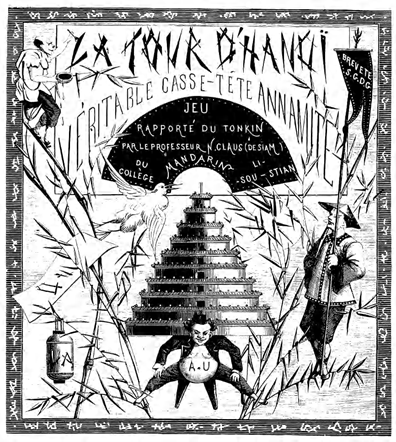
\includegraphics[width=0.4\textwidth]{1.1}
		\caption{\small\textit{\color{hoccungpi}Hình $1$.}}
		\vspace*{-10pt}
	\end{figure}
	Khi đó ta có các kết quả sau:
	\begin{align*}
		OI^2=R(R-2r), \tag{$2$}\\
		OH^2=9R^2-a^2-b^2-c^2,  \tag{$3$}\\
		IA+IB+IC\ge 6r, \tag{$4$}\\
		OH\ge OI,\tag{$5$}\\
		r=R(\cos{A}+\cos{B}+\cos{C}-1). \tag{$6$}
	\end{align*}
	Công thức ($2$) là hệ thức Euler, [$6$, pp. $186-187$]. Công thức ($3$) là một kết quả cơ bản trong tam giác [$4$, p. $31$]. Ta có thể chứng minh ($5$) dựa vào ($2$) và ($3$) như sau. Ta có 
	\begin{align*}
		OH^2-OI^2&=8R^2+2Rr-(a^2+b^2+c^2)\\
		&\ge 8R^2+4r^2- (a^2+b^2+c^2)\\
		&\ge 0,
	\end{align*}
	theo bất đẳng thức Euler $R\ge 2r$ và bất đẳng thức Gerretsen [$2$] $a^2+b^2+c^2\le 8R^2+4r^2$. Suy ra $OH\ge OI$.
	Đẳng thức xảy ra khi tam giác $ABC$ đều.
	\vskip 0.05cm
	Bất đẳng thức ($4$) là hệ quả của bất đẳng thức Erd\H{o}s--Mordell [$3$], áp dụng cho điểm $I$; đẳng thức xảy ra khi tam giác $ABC$ đều.
	\vskip 0.05cm
	Ngoài ra, nếu tam giác $ABC$ là nhọn thì:
	\begin{align*}
		OD+OE+OF=R+r, \tag{$7$}   \\ 
		HA+HB+HC=2R+2r,    \tag{$8$}
	\end{align*}
	Đẳng thức ($7$), còn gọi là công thức Carnot (đúng cho mọi tam giác nhọn [$5$, p. $83$]).  
	Ta chỉ sử dụng ($6$) trong phần $3$.
	Chú ý rằng tất cả chứng minh trên, ngoài trừ cho ($6$) và ($4$), đều là chứng minh hình học. 
	\vskip 0.05cm
	$\pmb{2.}$ \textbf{\color{hoccungpi}Một chứng minh hình học cho $\pmb{(1)}$}
	\begin{figure}[H]
		\vspace*{-5pt}
		\centering
		\captionsetup{labelformat= empty, justification=centering}
		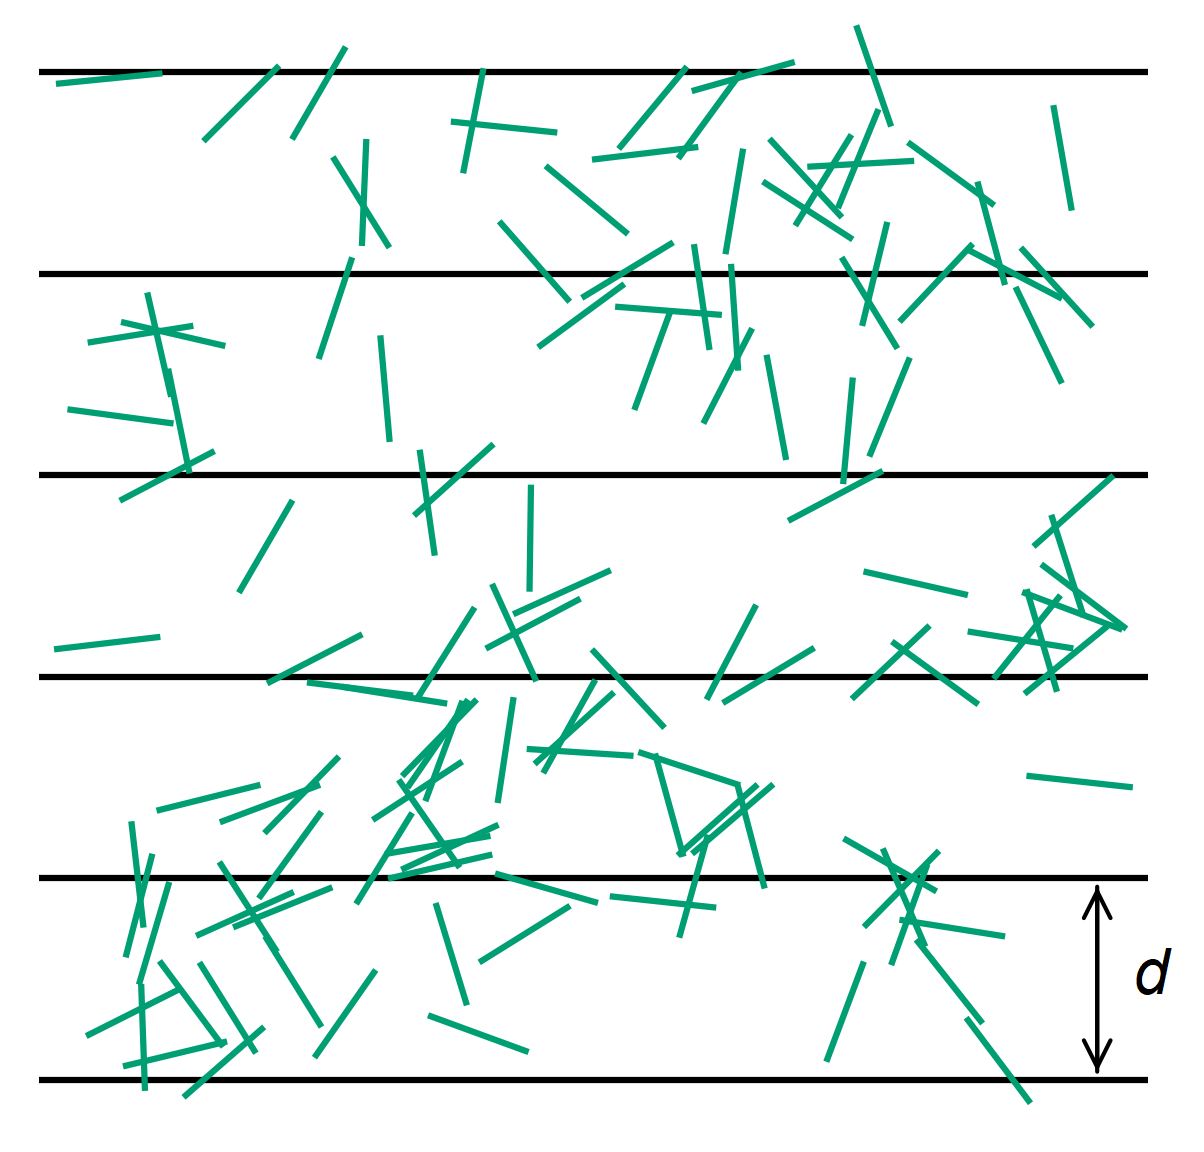
\includegraphics[width=0.35\textwidth]{2}
		\caption{\small\textit{\color{hoccungpi}Hình $2$.}}
		\vspace*{-10pt}
	\end{figure}
	Bây giờ ta sẽ đưa ra chứng minh hình học cho ($1$).
	\vskip 0.05cm
	Gọi $R_1$ và $r_1$ tương ứng là bán kính đường tròn ngoại tiếp và nội tiếp của tam giác  $I_AI_BI_C$.
	Gọi $M,N,P$ tương ứng là trung điểm của $I_BI_C,I_CI_A,I_AI_B$. Gọi $O_1,O$ lần lượt là tâm đường tròn ngoại tiếp của tam giác $I_AI_BI_C$ và $ABC$. Khi đó tâm đường tròn Euler của tam giác $I_AI_BI_C$ là tâm đường tròn ngoại tiếp của tam giác $ABC$ và tam giác $MNP$. Chú ý rằng $I$ là trực tâm của tam giác $I_AI_BI_C$, nên $O$ là trung điểm của $IO_1$. Gọi $I_1$ và $r_2$ là tâm và bán kính đường tròn nội tiếp của tam giác $MNP$. Ta có $R_1=2R$ và $r_1=2r_2$. Chú ý rằng tam $I_AI_BI_C$ nhọn do $\angle I_A= \frac{\pi}{2}-\frac{\angle A}{2},  \angle I_B= \frac{\pi}{2}-\frac{\angle B}{2}, \angle I_C= \frac{\pi}{2}-\frac{\angle C}{2}$. Suy ra, từ ($8$) ta có 
	\begin{align*}
		II_A+II_B+II_C=4(R+r_2). \tag{$9$}
	\end{align*}
	Từ ($4$), ta có 
	\begin{align*}
		IA+IB+IC\ge 6r.
	\end{align*}
	Vì thế,
	\begin{align*}
		&A I_A + B I_B + C I_C \\
		= \,&AI + II_A+ BI + II_B+ + BI +II_C\\
		\ge \,&4R + 6r+ 4r_2.
	\end{align*}
	Do đó để chứng minh ($1$), ta chỉ cần chỉ ra
	\begin{align*}
		r_2\ge r. \tag{$10$}
	\end{align*}
	Do $I_1$ là tâm nội tiếp của tam giác $MNP$ và $I$ là tâm nội tiếp của tam giác $ABC$, nên theo ($2$) ta có
	\begin{align*}
		OI^2&=R(R-2r),\\
		OI_1^2&=R(R-2r_2).
	\end{align*}
	Suy ra, ($10$) tương đương với 
	\begin{align*}
		OI\ge OI_1. \tag{$11$}
	\end{align*}
	Chú ý rằng $O_1$ là trực tâm của tam giác $MNP$. Tâm $O$ của đường tròn ngoại tiếp tam giác $MNP$ là tâm của đường tròn Euler của tam giác $I_AI_BI_C$. Áp dụng ($5$) cho tam giác $MNP$,  có tâm đường tròn ngoại tiếp $O$, trực tâm $O_1$ và tâm đường tròn nội tiếp $I_1$, ta có $OO_1\ge OI_1$. Suy ra, $OI=OO_1\ge OI_1$. Do đó ($11$) đúng. Suy ra ($10$) đúng. Chứng minh hoàn tất.
	\vskip 0.05cm
	$\pmb{3.}$ \textbf{\color{hoccungpi}Phỏng đoán của Lukarevski}
	\vskip 0.05cm
	Bây giờ ta xét bất đẳng thức
	\begin{align*}
		\alpha R\!+\!(18\!-\!2\alpha)r\!\le\! AI_A\!+\!BI_B\!+\!CI_C \tag{$12$}
	\end{align*}
	với một hằng số $\alpha$, $4\le \alpha\le 9$, nào đó. Lukarevski phỏng đoán rằng ($12$) không đúng (với mọi tam giác $ABC$) với $\alpha=5$. Trong phần này, ta sẽ xây dựng ví dụ để chỉ ra rằng ($12$) không đúng trong trường hợp $\alpha>4$. Nói riêng, điều này cho thấy phỏng đoán của Lukarevski là đúng và hằng số $\alpha=4$ là tốt nhất có thể.
	\vskip 0.05cm
	Chú ý rằng theo ($9$) ta có 
	\begin{align*}
		AI_A\!+\!BI_B\!+\!CI_C\!=\!&IA\!+\!IB\!+\!IC\!+\!II_A\!+\!II_B\!+\!II_C\\
		=&IA\!+\!IB\!+\!IC\!+\!4R\!+\!4r_2.
	\end{align*}
	Suy ra, ($12$) tương đương với
	\begin{align*}
		&4r_2+IA+IB+IC\\[-0.5ex]
		\ge \,&(\alpha-4)R+(18-2\alpha)r.\tag{$13$}
	\end{align*}
	Để cho gọn, ta sẽ viết $\angle{M}$, $\angle{N}$, $\angle{P}$ thay cho $\angle{PMN}$, $\angle{MNP}$, $\angle{MPN}$, và viết $\angle{A}$, $\angle{B}$, $\angle{C}$ thay cho $\angle{BAC}$, $\angle{ABC}$, $\angle{BCA}$. Cho $R=1$, $\angle{B}=\angle{C}=x$, với $0<x<\dfrac{\pi}{2}$. Khi đó $\angle{A}=\pi-2x$. Suy ra, $\angle{M}=x$, $\angle{N}=\angle{P}=\dfrac{\pi}{2}-\dfrac{x}{2}$. Nên
	\begin{align*}r_2&=R(\cos{M}+\cos{N}+\cos{P}-1)\\[-0.5ex]
		&=2\sin{\dfrac{x}{2}}+\cos{x}-1,\\[-0.5ex]
		r&=R(\cos{A}+\cos{B}+\cos{C}-1)\\[-0.5ex]
		&=2\cos{x}-\cos{2x}-1\\[-0.5ex]
		&=2\cos{x}-2\cos^2{x}=4\cos{x}\sin^2{\dfrac{x}{2}},\\[-0.5ex]
		IA&=\dfrac{r}{\sin{\dfrac{A}{2}}}=4\sin^2{\dfrac{x}{2}},\\[-0.5ex]
		IB&=IC=\dfrac{r}{\sin{\dfrac{B}{2}}}=4\cos{x}\sin{\dfrac{x}{2}}.
	\end{align*}
	Suy ra, từ ($13$) ta có 
	\begin{align*}
		&4(2\sin\!{\dfrac{x}{2}}\!+\!\cos{x}\!-\!1\!\!)\!+\!4\sin\!{\dfrac{x}{2}}(2\cos{x}\!+\!\sin{\dfrac{x}{2}})\\[-0.5ex]
		\ge \,&\alpha-4+4(18-2\alpha)\cos{x}\sin^2{\dfrac{x}{2}}. \tag{$14$}
	\end{align*}
	Lấy giới hạn khi $x\rightarrow 0^{+}$ cho hai vế của ($14$) ta có
	\begin{align*}
		0 \ge \alpha-4.
	\end{align*}     
	Suy ra $\alpha \le 4$. Do đó ta kết luận rằng $4R+10r\le AI_A+BI_B+CI_C$ là bất đẳng thức tốt nhất.
	\vskip 0.05cm
	\textbf{\color{hoccungpi}Tài liệu}
	\vskip 0.05cm
	[$1$] M.~Lukarevski,~{An inequality for the altitudes of the excentre triangle,}~\textit{Math.~Gaz}, $\pmb{104}$ ($2020$), $161-164$.
	\vskip 0.05cm
	[$2$] M.~Lukarevski,~{An alternative proof of Gerretsen's inequalities,} \textit{Elem.~Math.} $\pmb{72}$, No. $1$ ($2017$), $2-8$.
	\vskip 0.05cm
	[$3$] C.~Alsina,~R.~B.~Nelson, A Visual Proof of the Erd\"{o}s--Mordell inequality, \textit{Forum Geometricorum,} $\pmb{7}$ ($2007$), $99-102$.
	\vskip 0.05cm
	[$4$] G.~Leversha, \textit{The Geometry of the Triangle}, UKTM ($2013$).
	\vskip 0.05cm
	[$5$] N.~Altshiller--Court,~\textit{College Geometry: An introduction to the Morden Geometry of the triangle and the circle,} Dover Publications ($2007$).
	\vskip 0.05cm
	[$6$] R.~A.~Johnson, \textit{Advanced Euclidean Geometry,} Dover Publications ($2007$).
\end{multicols}
\vspace*{-10pt}
\rule{1\linewidth}{0.1pt}
\begin{center}
	\vspace*{-5pt}
	\textbf{\Large\color{hoccungpi}LỜI GIẢI, ĐÁP ÁN}
	\vspace*{-5pt}
\end{center}
\begin{multicols}{2}
	$1$...Me$1+$ $2$.Vf$2$ Mc$2$ $3$.Xc$4$ Ma$3$ $4$.Xc$3$! Mb$1$ $5$.Xd$3$ Mã đen hết đường di chuyển.
	\vskip 0.05cm
	\textbf{\color{gocco}$\pmb{2}$.Xc$\pmb{4}$} [$2$.Xe$4+$ Cả hai phương án đều dẫn đến hòa cờ vì bên trắng không thể bắt được mã đen. $2$...Vf$5$ (\textit{$2$...Vd$5$})]
	\vskip 0.05cm
	\textbf{\color{gocco}$\pmb{2}$...Me$\pmb{1+}$ $\pmb{3}$.Vf$\pmb{2}$ Vd$\pmb{5!}$ $\pmb{4}$.Xc$\pmb{3}$ Vd$\pmb{4}$!} [Mã đen trốn thoát.]
	\vskip 0.05cm
	$1/2 -1/2$
	\vskip 0.05cm	
	\textbf{\color{gocco}Bài $\pmb{3}$: $\pmb{1}$.Mh$\pmb{6}$ Xh$\pmb{7}$ $\pmb{2}$.Mg$\pmb{8}$! Rb$\pmb{7}$ $\pmb{3}$.Mh$\pmb{6}$ Vf$\pmb{6}$ $\pmb{4}$.Mg$\pmb{8}$ Ve$\pmb{6}$ $\pmb{5}$.Mh$\pmb{6=}$}
	\vskip 0.05cm
	$1/2 -1/2$
	\vskip 0.05cm
	\textbf{\color{gocco}Bài $\pmb{4}$: $\pmb{1}$...Vf$\pmb{8}$! $\pmb{2}$.Xd$\pmb{7}$ Mg$\pmb{7}$ $\pmb{3}$.Vg$\pmb{6}$ Me$\pmb{8}$! $\pmb{4}$.Xf$\pmb{7+}$ Vg$\pmb{8}$ $\pmb{5}$.Xe$\pmb{7}$ Kf$\pmb{8}$! $\pmb{6}$.Xd$\pmb{7}$ Vg$\pmb{8}$! $\pmb{7}$.Xf$\pmb{7}$ Md$\pmb{6}$ $\pmb{8}$.Xf$\pmb{6}$ Me$\pmb{8}$! $\pmb{9}$.Xf$\pmb{1}$ Mg$\pmb{7}$ $\pmb{10}$.Vf$\pmb{6}$ Mh$\pmb{5+}$ $\pmb{11}$.Vg$\pmb{5}$ Mg$\pmb{7=}$ $\pmb{12}$.Vg$\pmb{6}$ Me$\pmb{8}$ $\pmb{13}$.Xf$\pmb{3}$ Mc$\pmb{7}$! $\pmb{14}$.Xf$\pmb{2}$} [$14$.Xc$3$ Me$8$ $15$.Xc$8$ Vf$8=$ Trắng không có cách nào bắt được mã đen]
	\vskip 0.05cm
	\textbf{\color{gocco}$\pmb{14}$...Ne$\pmb{8=}$} 
	\vskip 0.05cm
	$1/2 -1/2$
\end{multicols}